\chapter{State-space Control (LQG) of Stable Aircraft}
\section{Model Overview}
Figure \ref{fig:aircraft} represent a general aircraft longitudinal motion.
The dynamic model of the aircraft system \ref{fig:aircraft} is taken from
the article \cite{air_lqg}.

\begin{figure}[h]
    \centering
    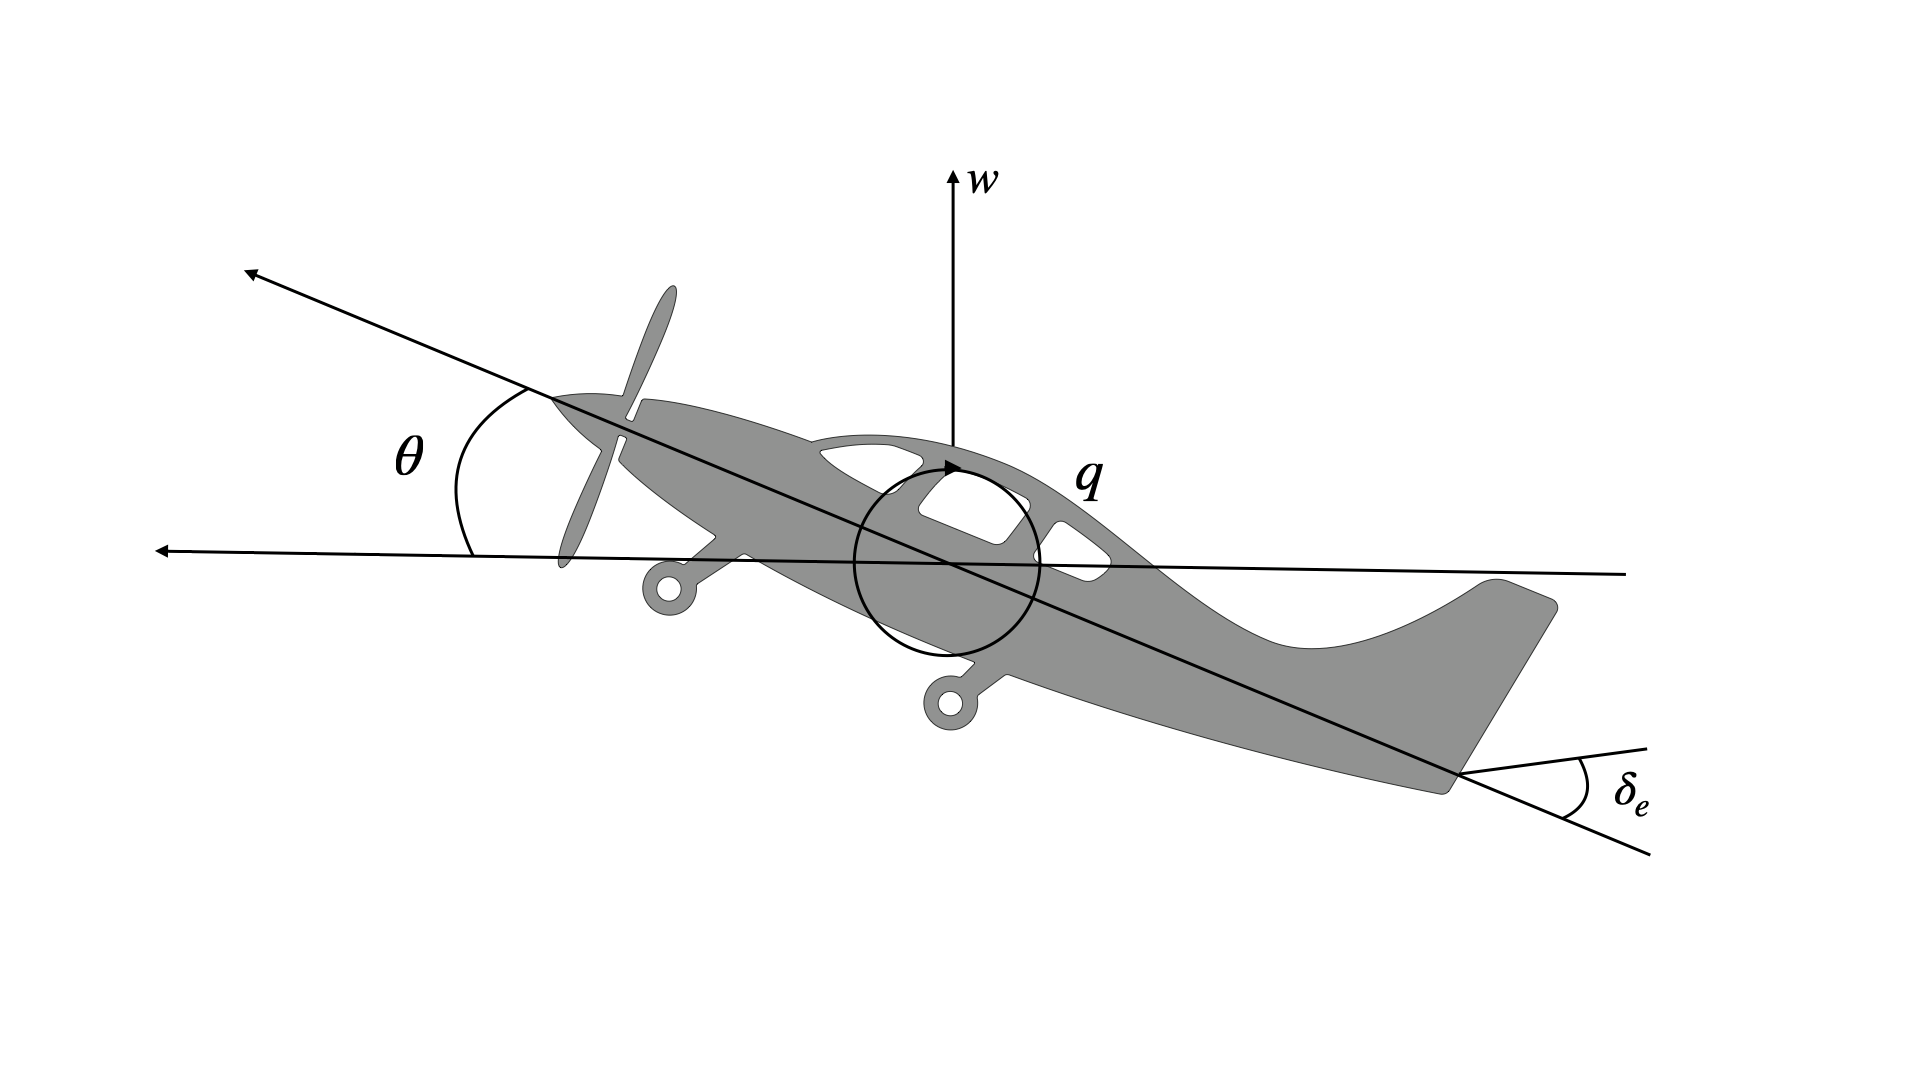
\includegraphics[width=0.6\textwidth]{aircraft.png}
    \caption{Aircraft longitudinal motion}
    \label{fig:aircraft}
\end{figure}


\begin{table}[h]
    \centering
    \begin{tabular}{|c|c|c|}
        \hline
        $\beta$     & rad         & Sideslip angle \\
        $p$         & rad/s       & Roll rate\\
        $r$         & rad/s       & Yaw rate\\
        $\Phi$      & rad         & Roll angle\\
        $w$         & m/s         & Vertical velocity\\
        $q$         & rad/s       & Pitch rate\\
        $\theta$    & rad         & Pitch angle\\
        $\delta_e$  & rad         & Elevator deflection\\
        \hline
    \end{tabular}
    \caption{System parameters}
    \label{tab:params}
\end{table}

\begin{tabular}{ |c|c| }
    \hline
    \hline
\end{tabular}

For longitudinal motion:
\begin{equation}
    \beta = p = r =\Phi = 0
\end{equation}

The transfer function is represented in state-space form by matrices:
\begin{align} \label{sys_ss}
    \begin{split}
        \dot{x} &= Ax + Bu \\
        y &= Cx + Du
    \end{split}
\end{align}

$A = \begin{bmatrix} -0.3149 & 235.8928 & 0 \\
                     -0.0034 & -0.4282  & 0 \\
                      0      & 1        & 0 \end{bmatrix}$ \\


$B = \begin{bmatrix} -5.5079   \\
                      0.0021   \\
                      0        \end{bmatrix}$ \\


$C = \begin{bmatrix}  0 & 0 & 1 \end{bmatrix}$ \\


$D = 0$ \\

$x^T = \begin{bmatrix} w & q & \theta \end{bmatrix}$ \\

$u = \delta_e$

The implemented Model in Simulink is presented in the following 
diagram \ref{fig:plant}.

\begin{figure}[h]
    \centering
    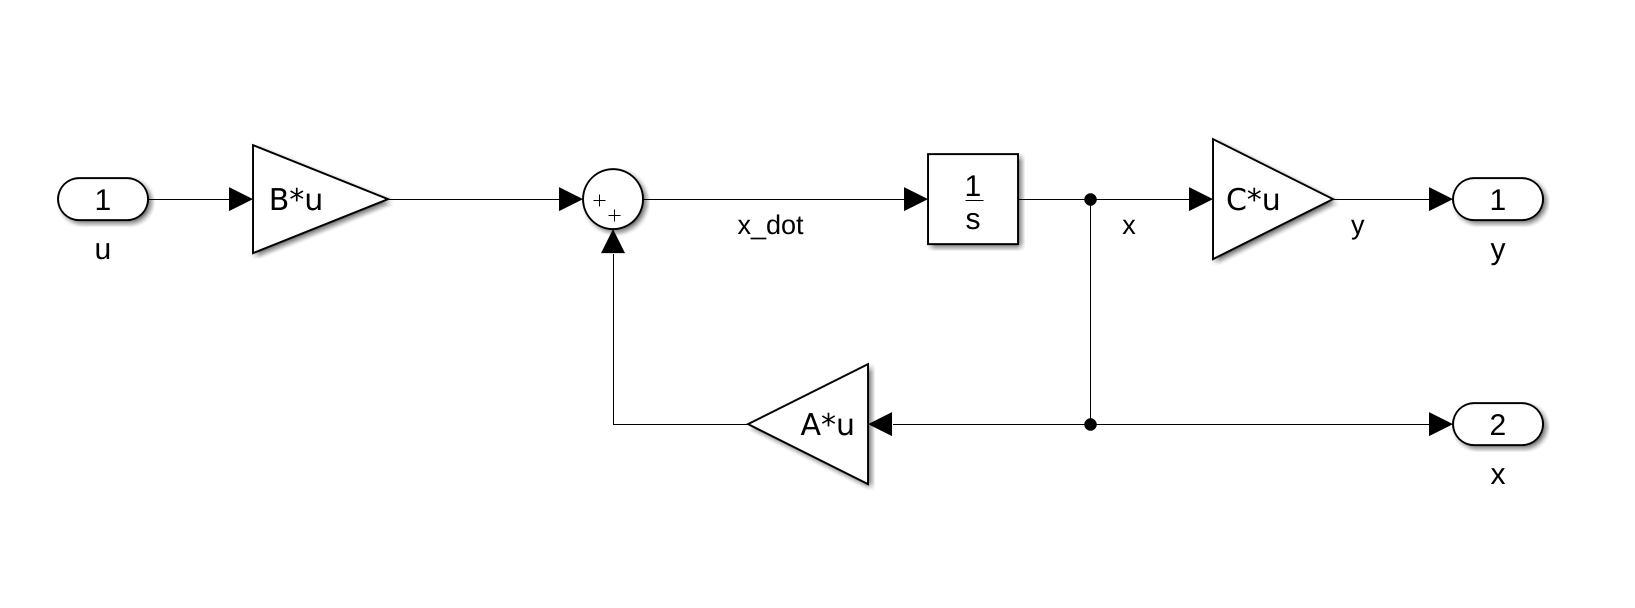
\includegraphics[width=0.6\textwidth]{plant.png}
    \caption{Plant model in Simulink.}
    \label{fig:plant}
\end{figure}

In the Matlab system can be represented by the state space function:
\begin{lstlisting}[frame=single]
>>sys = ss(A,B,C,D)
\end{lstlisting}

Figure \ref{fig:non_zero} represents the system behavior with non zero initial
conditions, where the pitch rate $q_0 = 1 \rm [rad/s]$.

\begin{figure}[h!]
    \centering
    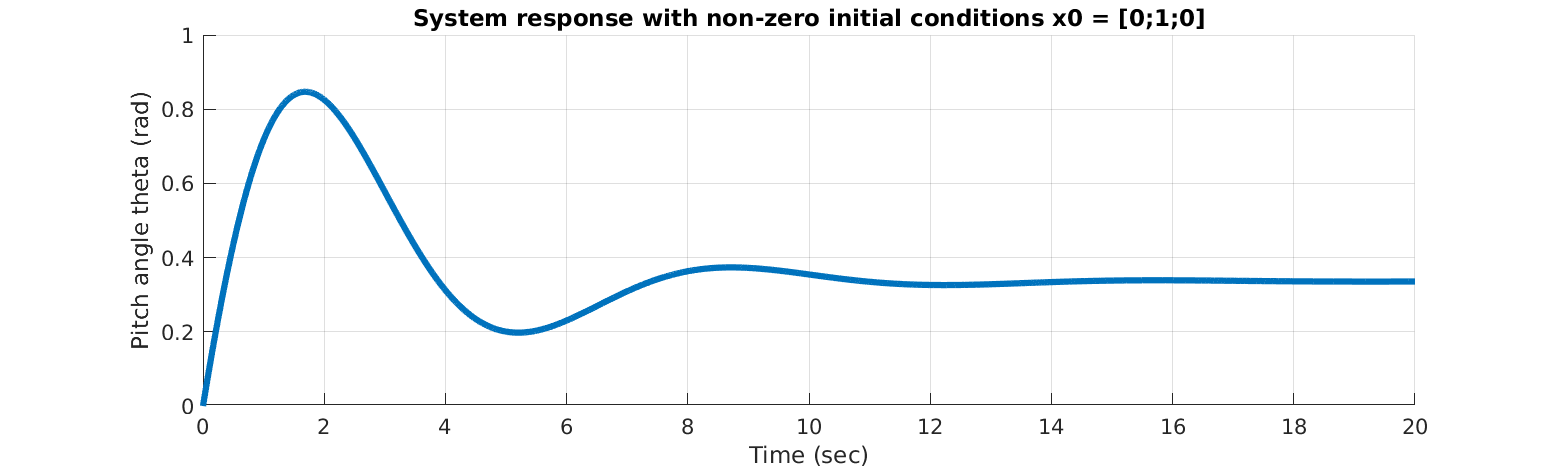
\includegraphics[width=1\textwidth]{non_zero.png}
    \caption{System response with non zero initial conditions}
    \label{fig:non_zero}
\end{figure}




\section{Open-loop Response}
The system is stable only if all the real parts of the eigenvalues are
negative. \\
The dynamics of the model is determined by the following parameters:\\
\textbf{Pols:}
\begin{align*}
   0.0000 + 0.0000i \\
  -0.3715 + 0.8938i \\
  -0.3715 - 0.8938i \\
\end{align*}
The real parts of eigenvalues are negative. The system is \textbf{stable}.\\
\textbf{Controllability matrix rank: $3$} \\
If the rank of Controllability matrix $Co = [ B\ AB\ A^2B\ \dots\ A^{n-1}B ]$
is equal to $n$ (number of states), the system is \textbf{controllable}. \\
\textbf{Observability matrix rank: $3$} \\
If the rank of Observability matrix $O = [ C\ CA\ CA^2\ \dots\ CA^{n-1} ]$
is equal to $n$, the system is \textbf{observable}.

The whole system is described by \ref{sys_ss} equations.
Open-loop impulse and step responses are presented in the figure
\ref{fig:open_loop}. The result corresponds to our expectations.

\begin{figure}[h!]
    \centering
    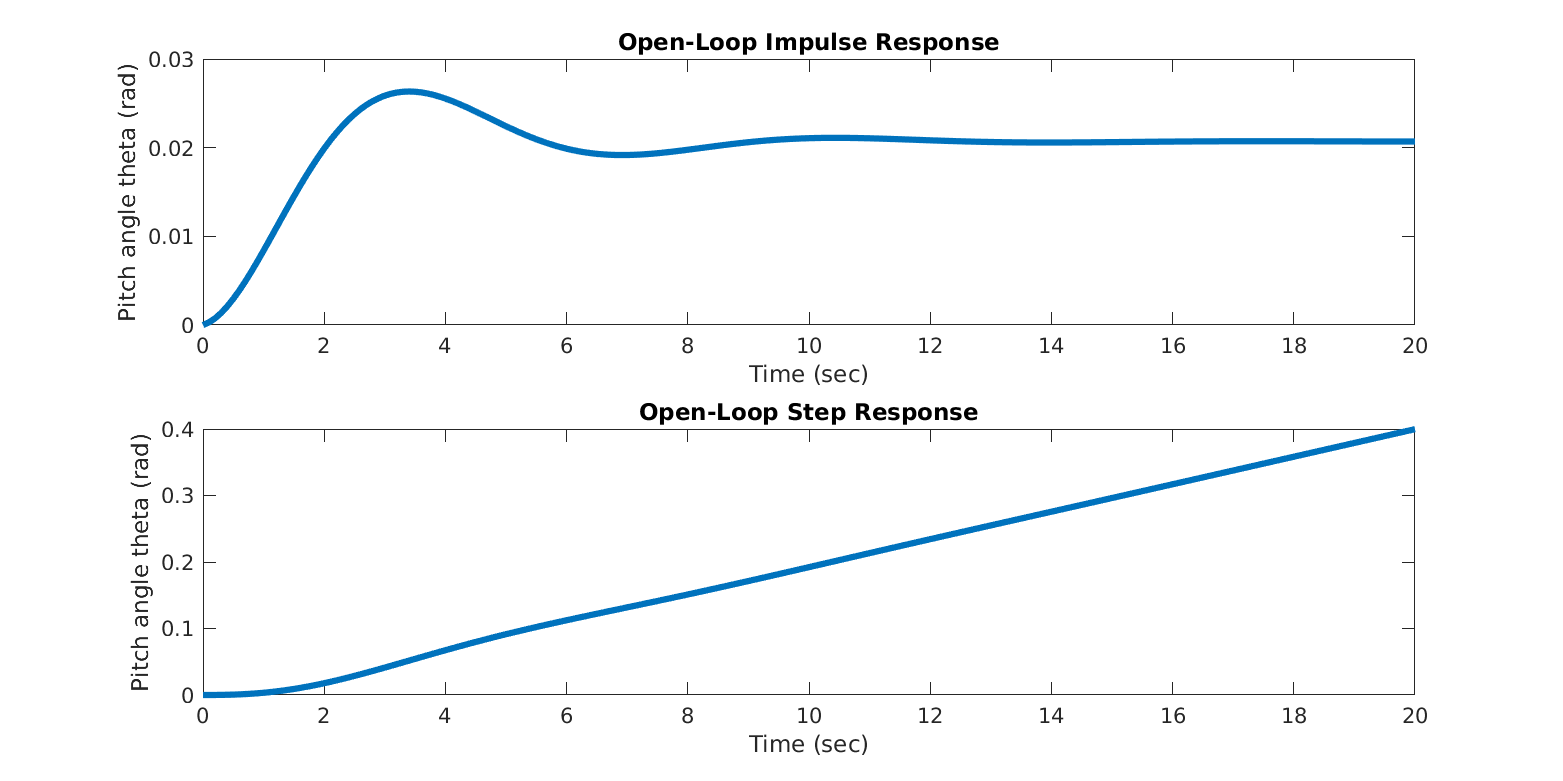
\includegraphics[width=1\textwidth]{open_loop.png}
    \caption{Open-loop system response}
    \label{fig:open_loop}
\end{figure}


\pagebreak

\section{LQR Design - zero control}
In modeling zero control response, the input of the system
will be $u = -Kx$, ($r=0$). Substituting into equation \ref{sys_ss}, the
result of Close-loop system will correspond to equation \ref{sys_cl}.

\begin{align}\label{sys_cl}
    \dot{x} = (A-BK)x
\end{align}

For calculation $K$ gain were used LQR method. This method based on quadratic
cost function $J$. Where $Q$ matrix represent how "fast" controller will approximate 
the following state. 
$R$ matrix represent how much we depend on energy that we add to system to
control.
\begin{equation}
J=\int(x^TQx + u^TRu)dt
\end{equation}


In Matlab we define Q and R matrix and use a \textbf{lqr} command.
\begin{lstlisting}[frame=single]
Q = diag([0, 0, 500]);
R = .1;
K = lqr(A,B,Q,R);
\end{lstlisting}

Simulink model of close-loop system is presented in the following diagram
\ref{fig:zero_control}.

\begin{figure}[h]
    \centering
    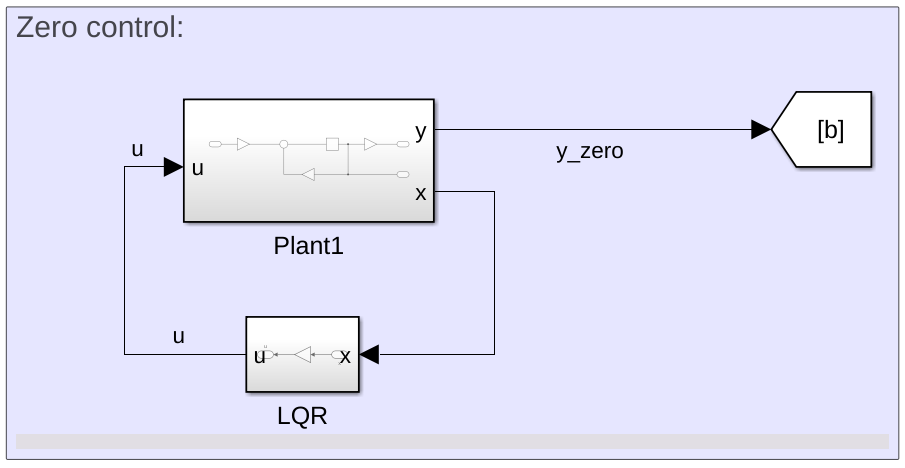
\includegraphics[width=0.6\textwidth]{zero_control.png}
    \caption{Zero control model in Simulink.}
    \label{fig:zero_control}
\end{figure}

Figure \ref{fig:zero_control} represent the system behavior controlled by
LQR controller with non-zero initial conditions.

\begin{figure}[h!]
    \centering
    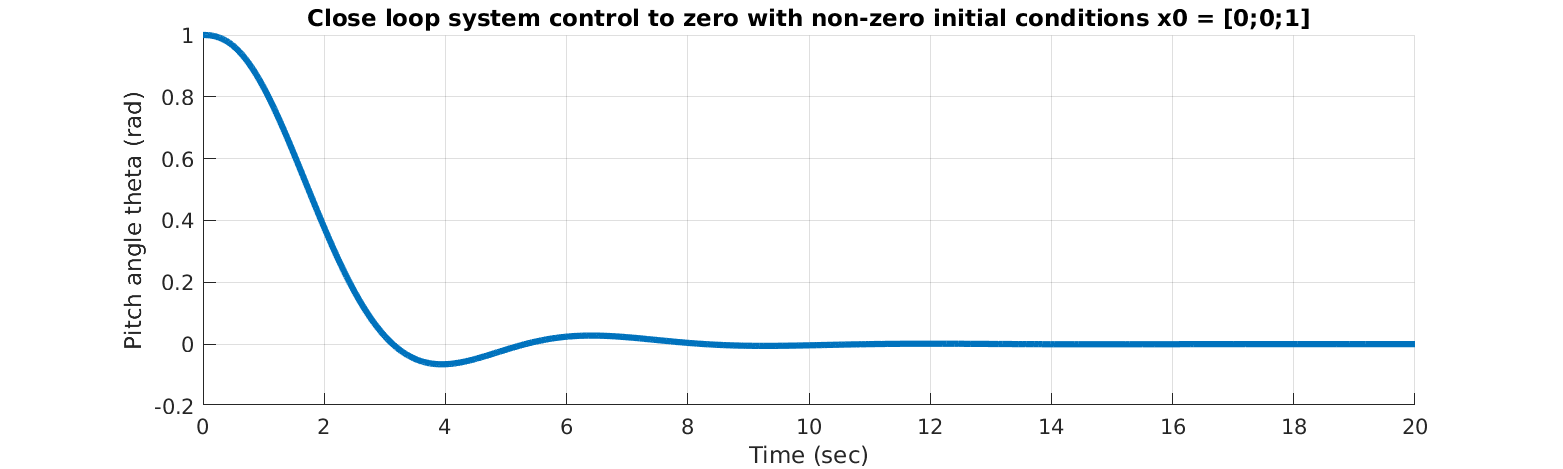
\includegraphics[width=1\textwidth]{control2zero.png}
    \caption{Zero control with non-zero initial conditions}
    \label{fig:zero_control}
\end{figure}


\section{LQR Design - control to the point - rscale}

$N$ gain is used to scalar our input for a full-state feedback system to 
eliminate the steady-state error.
\begin{equation}\label{r_n}
    u = -Kx + rN
\end{equation} 
where $r$ is final point. Substituting equation \ref{r_n} into equation \ref{sys_ss}, the
result of Close-loop system controlled to $r$ will correspond to equation
\ref{BNr}.
\begin{equation}\label{BNr}
    \dot{x} = (A-BK)x + BNr
\end{equation}

For calculation \textbf{N} gain in Matlab were used \textit{rscale} function from
\cite{rscale}. 
\begin{lstlisting}[frame=single]
N = rscale(A,B,C,D,K);
\end{lstlisting}

Simulink model of Close-loop system controlled to point is presented in the
following diagram \ref{fig:model_to_point}.

\begin{figure}[hbt!]
    \centering
    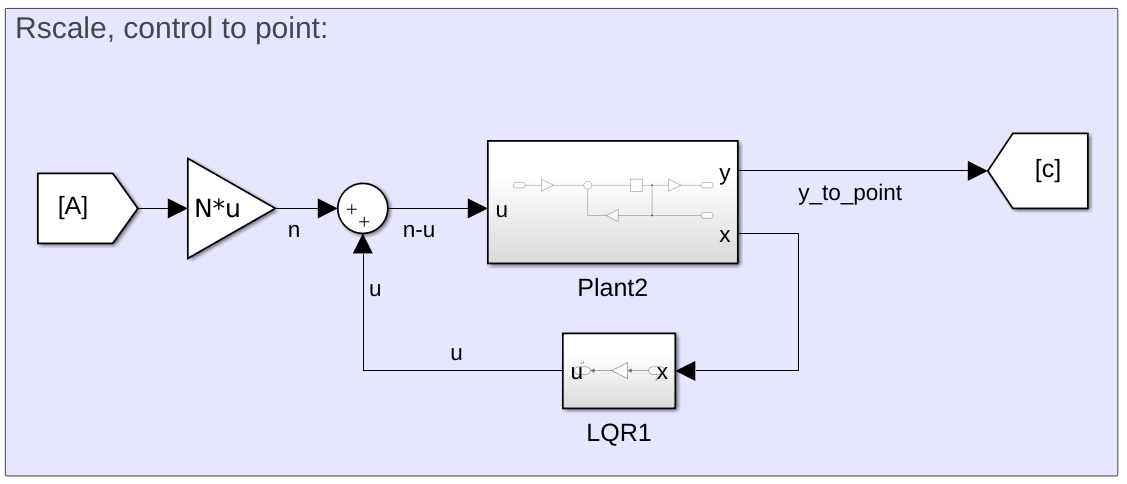
\includegraphics[width=0.6\textwidth]{model_to_point.png}
    \caption{Rscale control to point model in Simulink.}
    \label{fig:model_to_point}
\end{figure}

In the Matlab system can be represented by the state space function:
\begin{lstlisting}[frame=single]
>>sys = ss(A-B*K,B*N,C,D)
\end{lstlisting}

The Close-loop impulse and step response are presented in the following
figure \ref{fig:close_loop}.

\begin{figure}[h!]
    \centering
    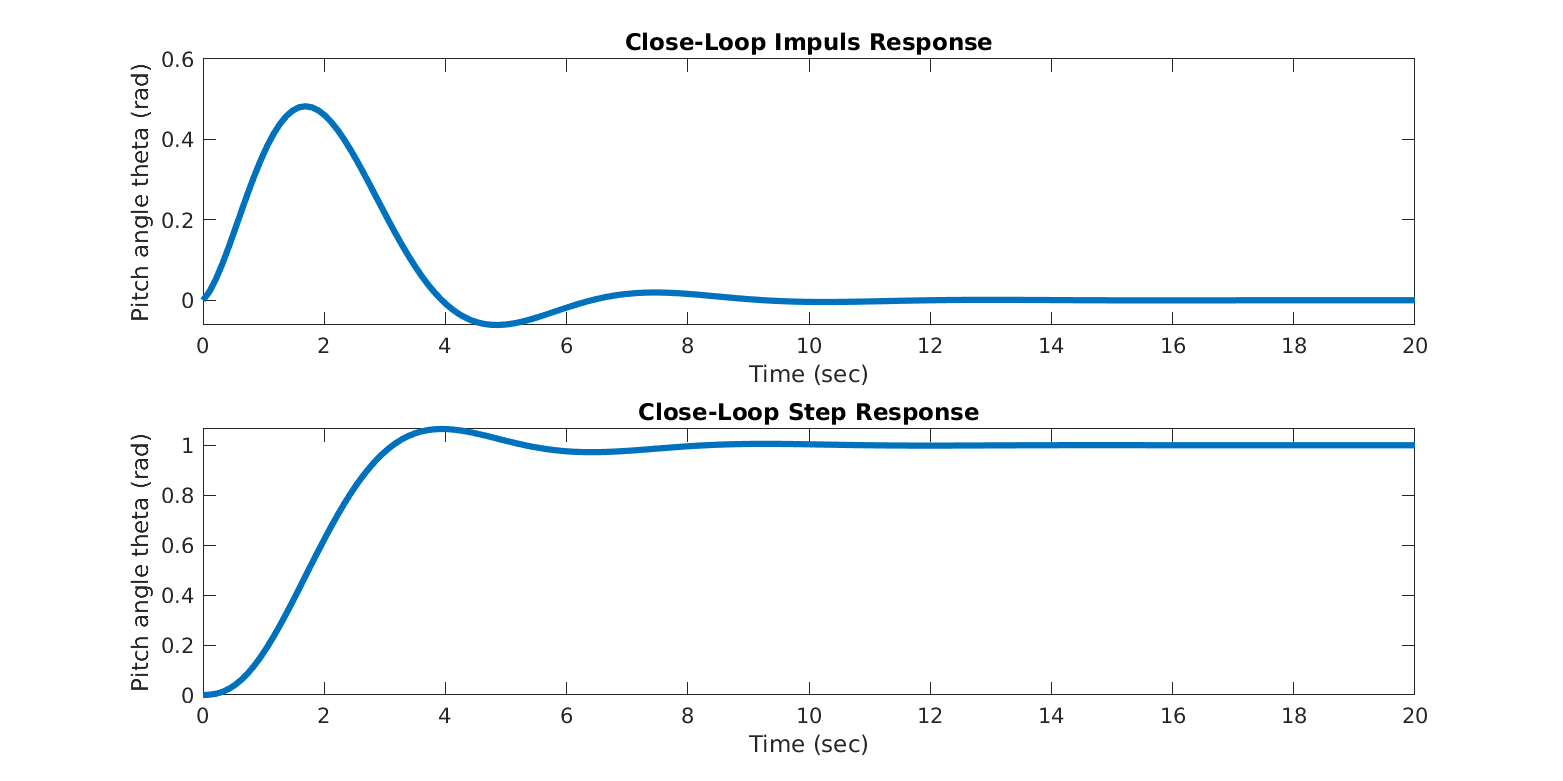
\includegraphics[width=1\textwidth]{close_loop.png}
    \caption{Close-loop impulse and step system responses}
    \label{fig:close_loop}
\end{figure}

\section{Study of System Behavior}

In case Longitudinal dynamic it's possible to measure $\theta$ (pitch
angle). At this moment, there is no specific conditions for deflector angle actuator. The
$R = 0.1$ matrix we will keep equal to 0.1. In the following figure
\ref{fig:diff_Q}, there are impulse responses for 
different $Q$ matrices. Where we change $x$ parameter from 1 to 500 with 50 as
step.


$Q = \begin{bmatrix}  0 & 0 & 0 \\
                      0 & 0 & 0 \\
                      0 & 0 & x \end{bmatrix}$ \\

\begin{figure}[hbt!]
    \centering
    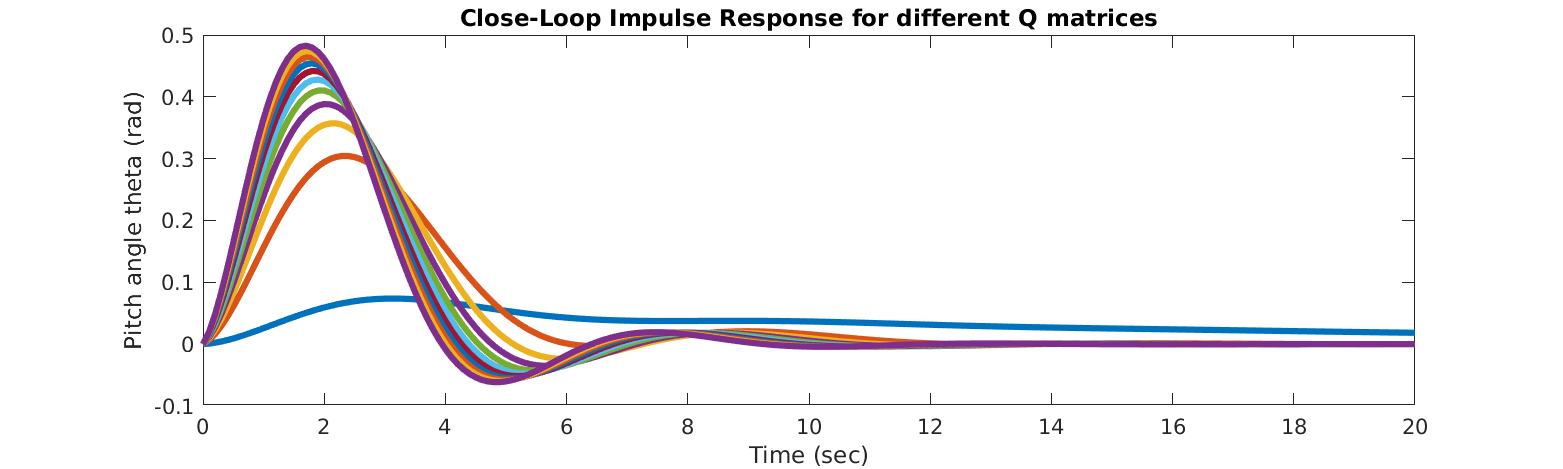
\includegraphics[width=1\textwidth]{lqr_diff_Q.png}
    \caption{Impulse response for different Q matrices.}
    \label{fig:diff_Q}
\end{figure}
The following Q and R matrices will suffice for our purposes. These values
will be used in the following simulations.

$Q = \begin{bmatrix}  0 & 0 & 0 \\
                      0 & 0 & 0 \\
                      0 & 0 & 500 \end{bmatrix}$  \
$R = 0.1$

\section{Acting Value Saturation}
It's very hard to find some examples of used actuators in aircraft field.
In this section different saturation values was studied.  However, in this
section we will try to see how different saturation values affect the
behavior of the system. Assuming that the elevator deflector $\delta_e$ 
possible positions are situated in range from 0.5 to 1.5 [rad].
Figure \ref{fig:sat_diff} present different system responses for different saturation
values in the range from 0.5 to 1.5 [rad].

\begin{figure}[h!]
    \centering
    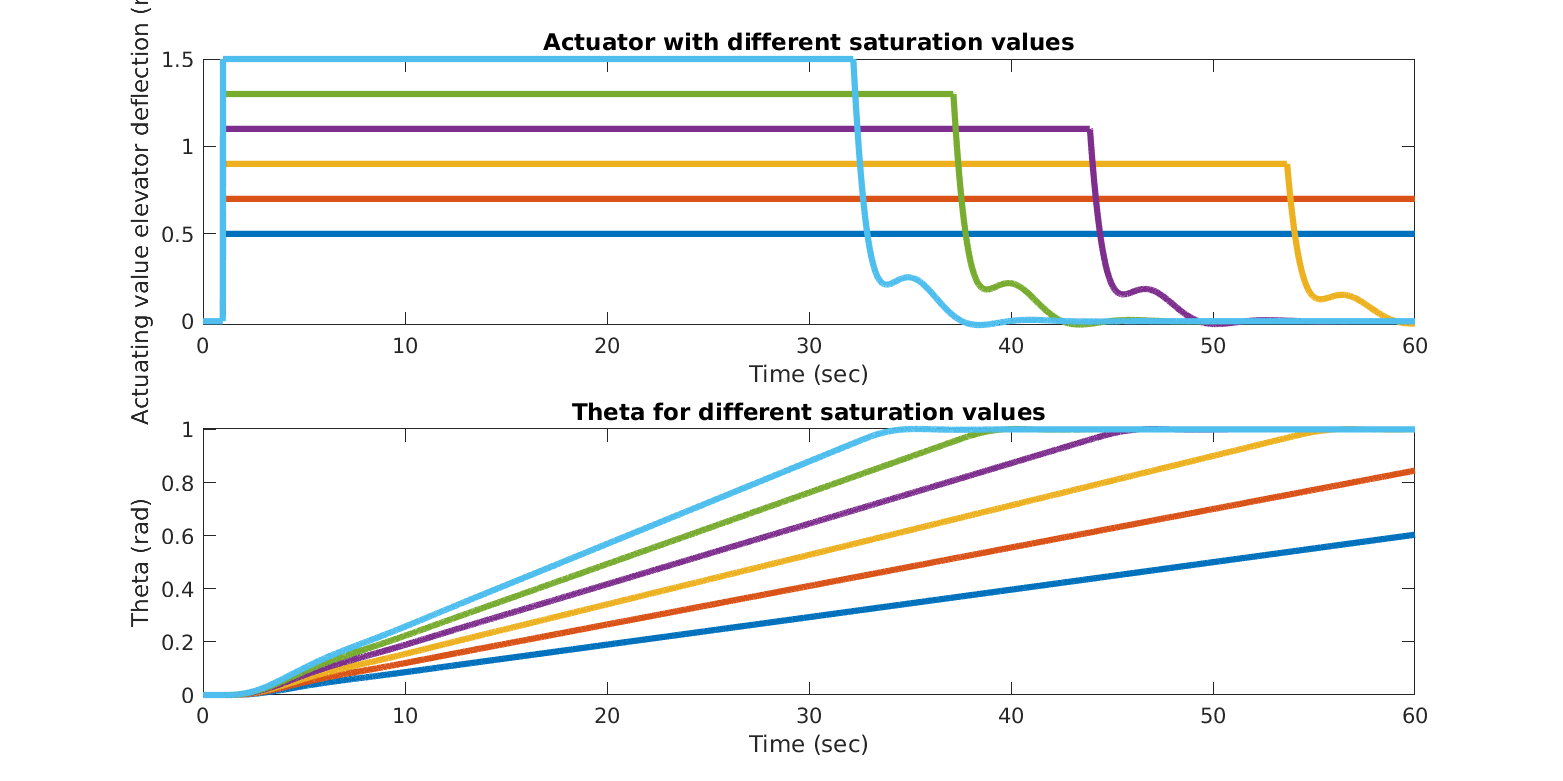
\includegraphics[width=1\textwidth]{lqr_saturation_diff.png}
    \caption{System response controlled LQR with different saturation values}
    \label{fig:sat_diff}
\end{figure}

At this step we will satisfying with fastest saturation value $1.5 \text{rad} \approx 90 ^o$. The system response with saturation 1.5 rad shown in figure \ref{fig:sat}.

\begin{figure}[h!]
    \centering
    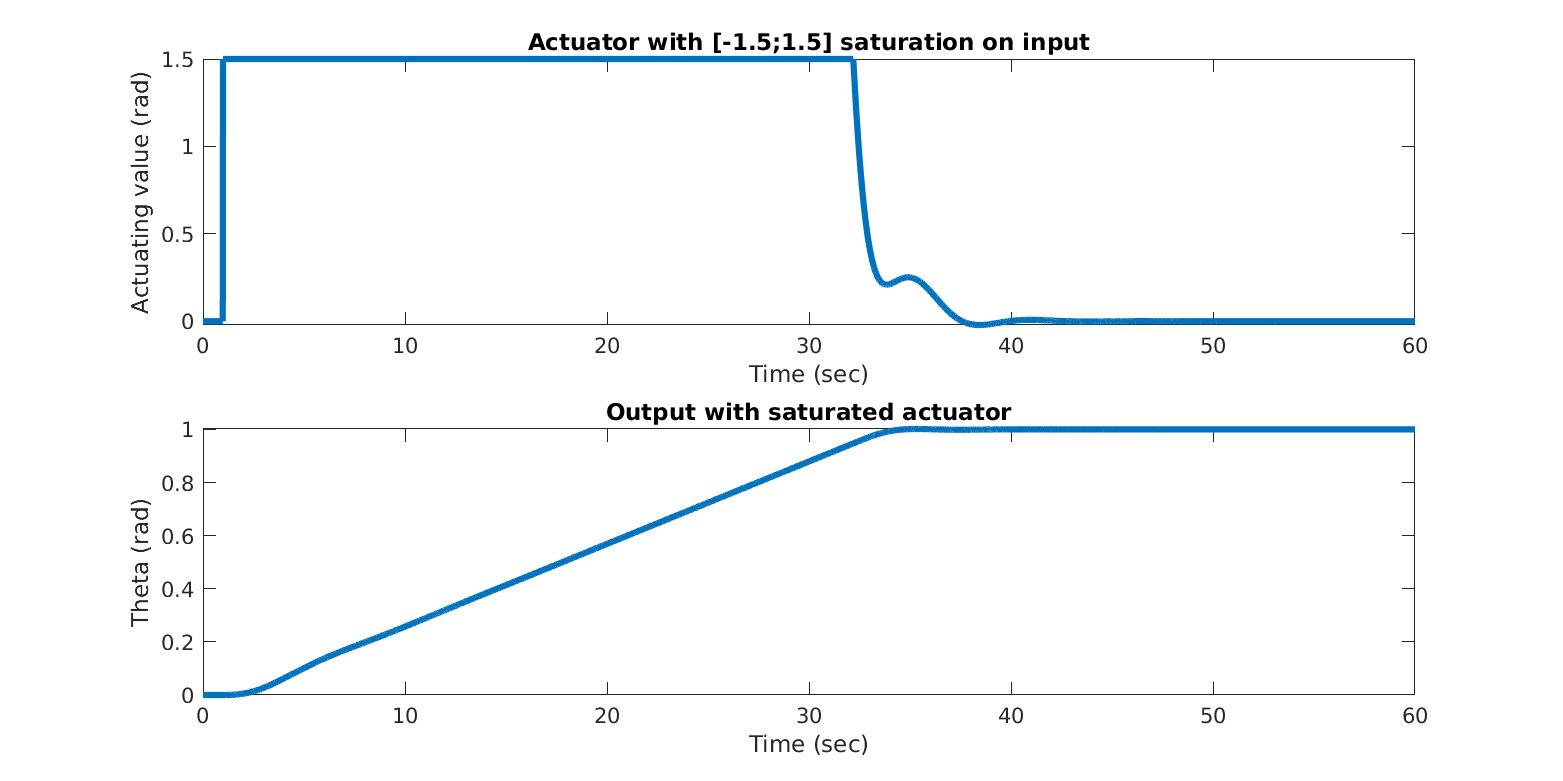
\includegraphics[width=1\textwidth]{lqr_saturation.png}
    \caption{System response with input saturation = 1.5 rad}
    \label{fig:sat}
\end{figure}

As we can see the aircraft dynamic in longitudinal motion with saturated
elevator deflection shows a sufficiently slow behavior, which, however,
corresponds to reality.





\section{Kalman Filter Implementation}
The LQR controller can be used if we have information about the whole
state $x$. A Kalman filter can be used to reconstruct the state from the
$y$ measurement. The following system of equations \ref{kf} representing Kalman filter.

\begin{equation}\label{kf}
    \begin{split}
        \frac{d}{dt}\hat{x} = A\hat{x} + Bu + Kf(y-\hat{y})\\
        \hat{y} = C\hat{x}
    \end{split}
\end{equation}


Simulink model of Kalman filter is presented in the following diagram
\ref{fig:kf_model}.

\begin{figure}[hbt!]
    \centering
    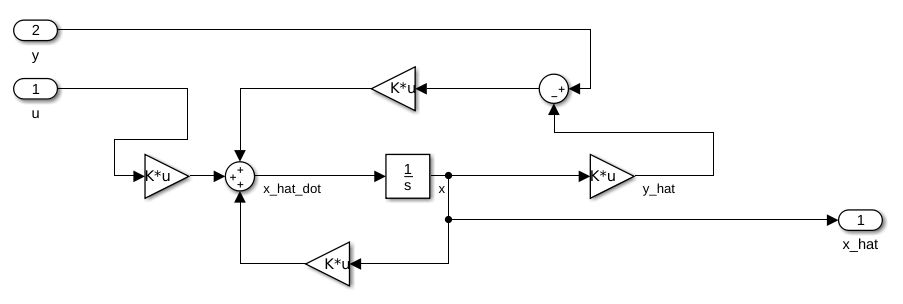
\includegraphics[width=0.6\textwidth]{kf_model.png}
    \caption{Kalman filter implementation in Simulink}
    \label{fig:kf_model}
\end{figure}

Kalman filter use knowledge  about disturbance of state and measurement
noise magnitudes. $Vd$ matrix representing covariance of state disturbance
and $Vn$ matrix is covariance of measurement noise.
There are more options how to calculate $Kf$ gain. Define $Vd$
and $Vn$ matrices we can use the same \textbf{lqr} function as follow: 

\begin{lstlisting}[frame=single]
Sw = .1;
Sv = 1;
[kalmf, Kf, P] = kalman(sys_ss, Sw, Sv); 
\end{lstlisting}

Simulink model of system is presented in the following diagram
\ref{fig:lqg}.

\begin{figure}[hbt!]
    \centering
    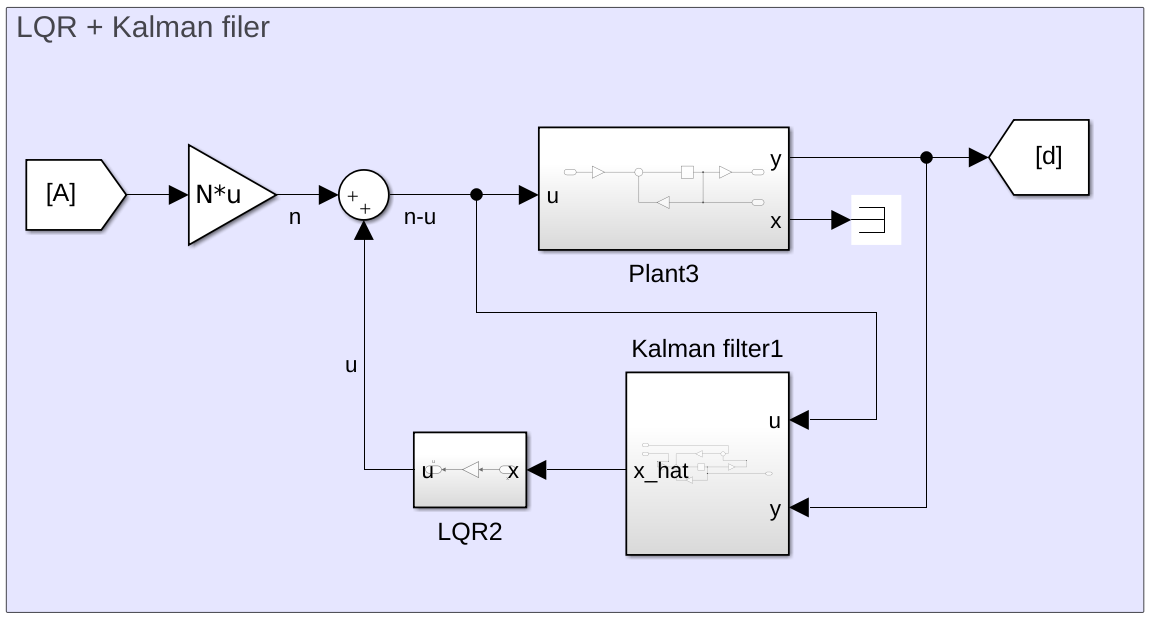
\includegraphics[width=0.6\textwidth]{model_lqr_kalman.png}
    \caption{Rscale control to point model in Simulink.}
    \label{fig:lqg}
\end{figure}

Implementing Kalman filter in Matlab:
\begin{lstlisting}[frame=single]
Akf = A-Kf*C;
Bkf = [B Kf];
Ckf = eye(3);
Dkf = 0*[B Kf];
sys_kf = ss(Akf, Bkf, Ckf, Dkf);
\end{lstlisting}

\section{Study of system behavior with an observer (simulation)}
The real system control contain measurement noise and disturbance. In model
\ref{fig:lqg_noise} were used $w_d$ and $w_n$ disturbance and noise inputs
as Gaussian white noise.


The whole system with LQG implementation, disturbances and noise can be
describe as following system of equations \ref{lqg_final}.
\begin{equation}
        \epsilon = x - \hat{x} \\
\end{equation}


\begin{equation}\label{lqg_final}
\begin{bmatrix} \dot{x} \\ \dot{\epsilon} \end{bmatrix}  = 
\begin{bmatrix} A-BK & BK \\ 0 & A-KfC \end{bmatrix} \cdot 
\begin{bmatrix} x \\ \epsilon \end{bmatrix} +
\begin{bmatrix} I & 0 \\
                I & -Kf
\end{bmatrix} \cdot
\begin{bmatrix} w_d \\ w_n \end{bmatrix}
\end{equation}

The whole model is controlled by placing eigenvalues in $A-BK$ and $A-KfC$
by $K$ and $Kf$ matrices. 
 

Simulink model is presented in the following diagram
\ref{fig:lqg_noise}.

\begin{figure}[hbt!]
    \centering
    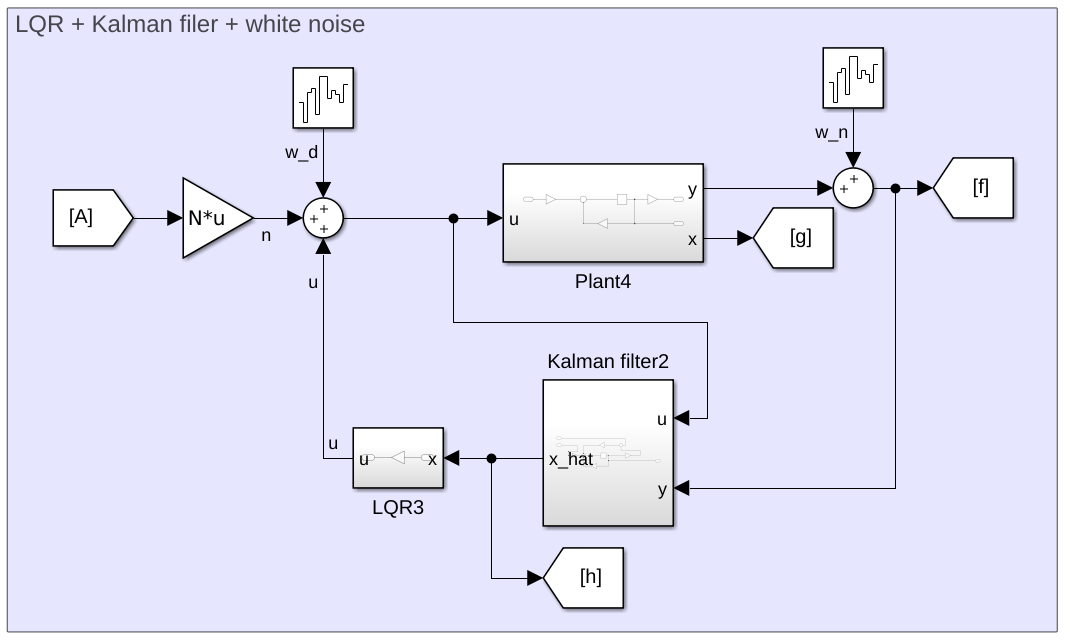
\includegraphics[width=0.6\textwidth]{lqg_noise.png}
    \caption{LQG simulink model}
    \label{fig:lqg_noise}
\end{figure}


The following graph \ref{fig:lqg_noise_plot} shows the correct operation
of the LQG controller. Kalman filter correctly estimates the state with
permissible noise level.

\begin{figure}[hbt!]
    \centering
    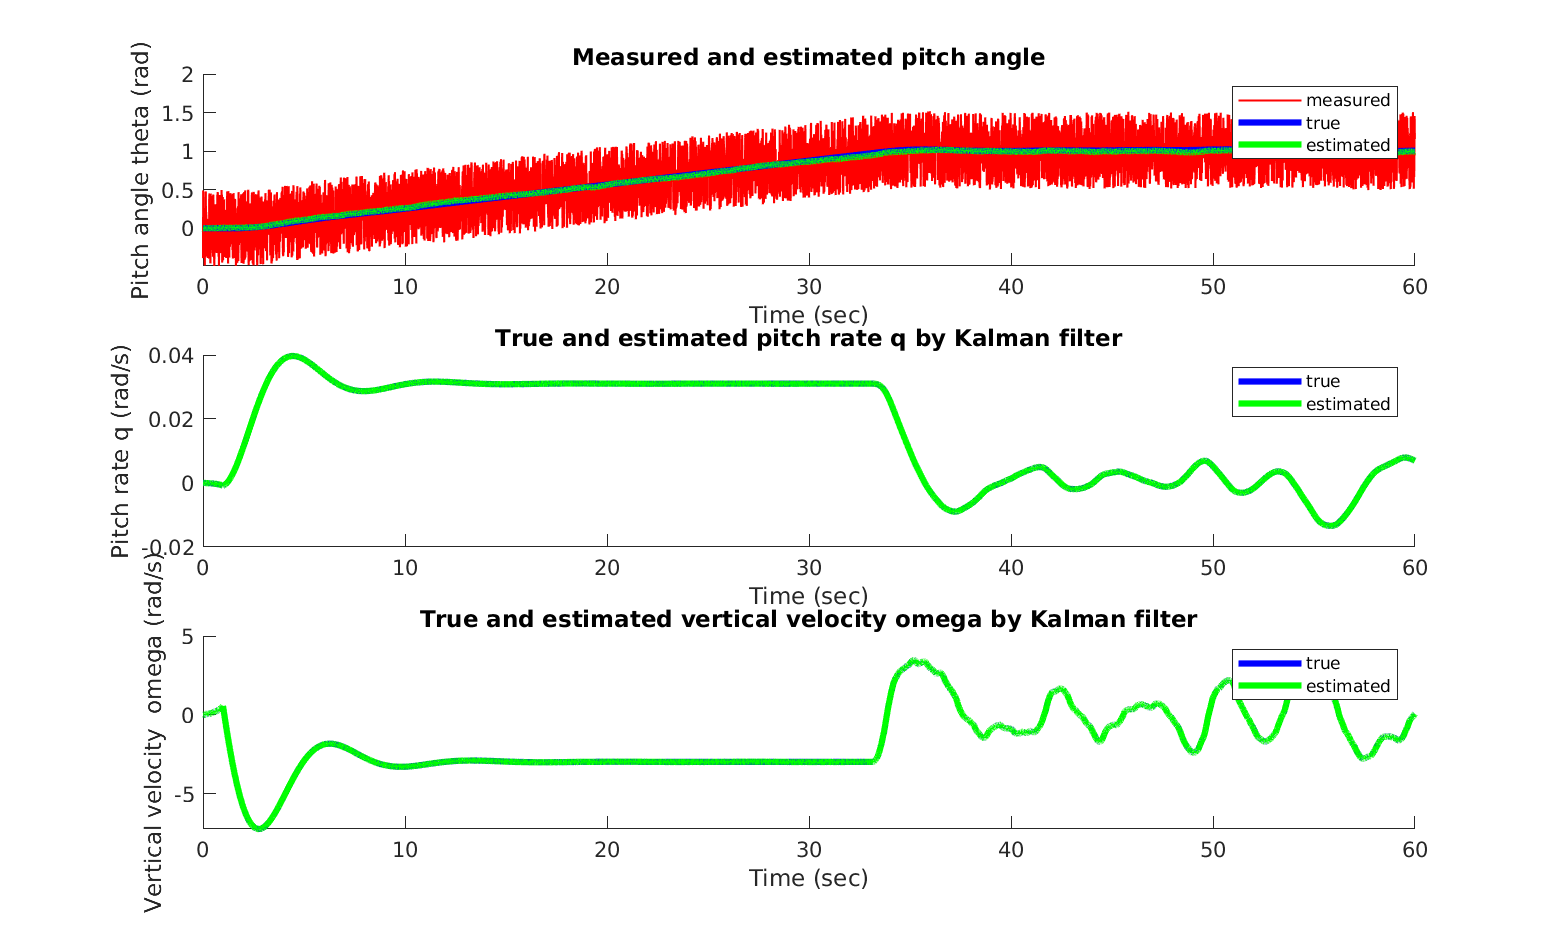
\includegraphics[width=1\textwidth]{lqg_saturated_noise.png}
    \caption{LQG regulator output}
    \label{fig:lqg_noise_plot}
\end{figure}

With increasing noise amplitude, the model is able to remain functional.
This can be verified by changing the disturbance and noise magnitude in the
Simulink model.

\section{Evaluation of the whole task and conclusion}
The aircraft model used in this task is stable, observable, and
controllable.  System behavior was studied, and an LQR regulator was added.
Using Kalman filter as state observer, LQG control was implemented. Using
saturation on the system's input with noisy measurement, LQG control is
still correctly working.  LQG can be used to control the pitch angle of an
aircraft and sufficiently resistant to the measurement noise.
Implementation in the Matlab/Simulink environment sufficiently clear and
easily salable.

All Simulink models and Matlab scripts are available in appendix.
